\documentclass[12pt,a4paper]{article}

\usepackage[margin=1in]{geometry}
\usepackage{amsmath,amssymb}
\usepackage{graphicx}
\usepackage{listings}
\usepackage{xcolor}
\usepackage{setspace}
\usepackage{titlesec}
\usepackage{caption}
\usepackage{hyperref}
\usepackage{url}
\usepackage{tikz}
\usetikzlibrary{positioning,arrows.meta,calc}

\onehalfspacing

% Python listing style
\lstset{
  language=Python,
  basicstyle=\ttfamily\small,
  keywordstyle=\color{blue}\bfseries,
  commentstyle=\color{gray!70!black}\itshape,
  stringstyle=\color{teal},
  numbers=left,
  numberstyle=\tiny\color{gray},
  stepnumber=1,
  numbersep=8pt,
  frame=single,
  breaklines=true,
  showstringspaces=false,
  tabsize=4,
  captionpos=b,
  xleftmargin=1.5em,
  framexleftmargin=1em,
  aboveskip=1.2em,
  belowskip=1em,
}

\titleformat{\section}{\large\bfseries}{\thesection}{1em}{}
\titleformat{\subsection}{\normalsize\bfseries}{\thesubsection}{1em}{}

\begin{document}

% ---------------------------------------------------------------------------
% Title Page
% ---------------------------------------------------------------------------
\begin{titlepage}
  \thispagestyle{empty}
  \centering
  \vspace*{2.5cm}

  {\LARGE\bfseries Assignment 1\par}
  \vspace{1.5cm}

  {\Large Course: Deep Learning\par}
  \vspace{0.8cm}

  {\large Instructor: Dr.\ Ali Irtaza\par}
  \vspace{0.5cm}

  {\large Department of Electrical Engineering\par}
  \vspace{0.3cm}

  {\large Institute of Space Technology\par}

  \vfill

  {\large Submitted by:\par}
  \vspace{0.3cm}
  {\Large Zawar Khan\par}

  \vspace{1.5cm}
  {\large \today\par}
\end{titlepage}

% ---------------------------------------------------------------------------
% Question 1
% ---------------------------------------------------------------------------
\section*{Q1.\ Function approximation with a deep neural network}

Use deep neural networks to estimate the functions
(a)~$f(x)=x^{2}$,
(b)~$f(x)=\sin(x)$, and
(c)~$f(x)=|x|^{2}$.
Try data sets of different sizes, e.g.\ 10, 25, 50, 100 points for each
function. Use $80\%$ of the data for training and $20\%$ for testing.

\begin{enumerate}
  \item[(a)] Plot the test and training error for different sizes of the data sets.
  \item[(b)] Try reversing the sign of the weights and observe the performance.
\end{enumerate}

\noindent\textit{Hint:} Consider starting with a two-layer network with 3 hidden
units with $\tanh$ activation and a linear output unit.

\subsubsection*{Forward equations and training objective}

The hidden units apply the hyperbolic tangent:
\begin{align}
  h_1 &= \tanh(w_1 x + b_1), \\
  h_2 &= \tanh(w_2 x + b_2), \\
  h_3 &= \tanh(w_3 x + b_3).
\end{align}
The output unit is \textbf{linear}: a weighted sum of the hidden activations
plus a bias,
\begin{equation}
  \hat{y}
    = W_1 h_1 + W_2 h_2 + W_3 h_3 + b_{\mathrm{out}}.
  \label{eq:q1out}
\end{equation}
 The training is done by minimising the \textbf{mean squared error} (MSE)
\begin{equation}
  \mathrm{MSE}
    = \frac{1}{N}\sum_{n=1}^{N}\bigl(\hat{y}_n - y_n\bigr)^{2}
    = \frac{1}{N}\sum_{n=1}^{N}\bigl(\hat{y}_n - f(x_n)\bigr)^{2}.
  \label{eq:q1mse}
\end{equation}
Reaching exactly zero MSE is not expected in practice; a small positive value
is an acceptable stopping region (limits to be set later). Moreover, Weights are initialised randomly:
hidden $(w_1,b_1)$, $(w_2,b_2)$, $(w_3,b_3)$ and output
$(W_1,W_2,W_3,b_{\mathrm{out}})$.

\subsubsection*{Network architecture (block diagram)}

Figure~\ref{fig:q1arch} shows one scalar input~$x$ (not counted as a layer),
one hidden layer with three $\tanh$ neurons, and one linear output~$\hat{y}$.

\begin{figure}[htbp]
  \centering
  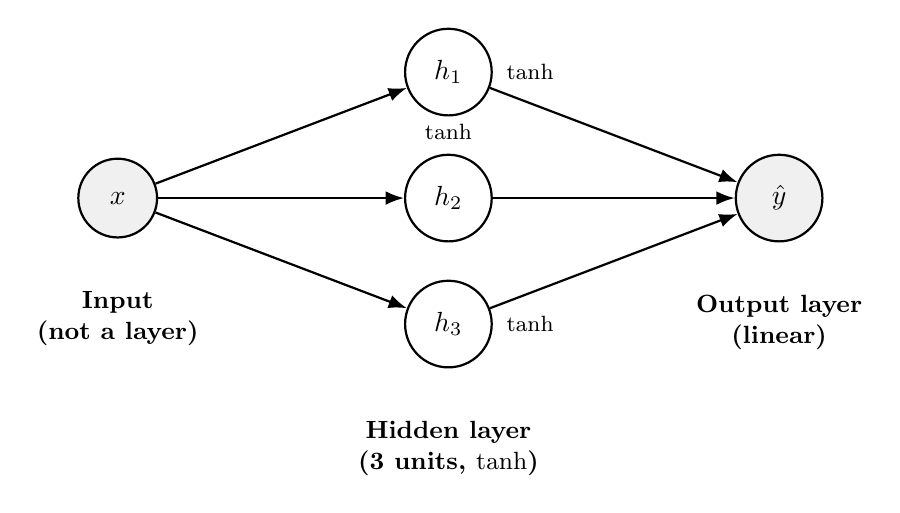
\begin{tikzpicture}[
      >=Latex,
      neuron/.style={circle, draw=black, thick, minimum size=11mm, inner sep=0pt},
      inputnode/.style={circle, draw=black, thick, minimum size=10mm, fill=gray!12},
      outputnode/.style={circle, draw=black, thick, minimum size=11mm, fill=gray!12},
      layerlabel/.style={font=\small\bfseries, align=center},
      note/.style={font=\footnotesize, align=center},
    ]
    % Input
    \node[inputnode] (x) at (0,0) {$x$};
    \node[layerlabel, below=0.55cm of x] {Input\\(not a layer)};

    % Hidden layer (3 units)
    \node[neuron] (h1) at (4.2, 1.6) {$h_1$};
    \node[neuron] (h2) at (4.2, 0.0) {$h_2$};
    \node[neuron] (h3) at (4.2,-1.6) {$h_3$};
    \node[layerlabel, below=0.55cm of h3] {Hidden layer\\(3 units, $\tanh$)};

    % Output
    \node[outputnode] (y) at (8.4, 0.0) {$\hat{y}$};
    \node[layerlabel, below=0.55cm of y] {Output layer\\(linear)};

    % Connections: input -> hidden
    \foreach \h in {h1,h2,h3} {
      \draw[->, thick] (x) -- (\h);
    }
    % Connections: hidden -> output
    \foreach \h in {h1,h2,h3} {
      \draw[->, thick] (\h) -- (y);
    }

    % Activation annotations
    \node[note, right=0.05cm of h1] {$\tanh$};
    \node[note, above=0.05cm of h2] {$\tanh$};
    \node[note, right=0.05cm of h3] {$\tanh$};
  \end{tikzpicture}
  \caption{Initial network for Q1: one input $x$, one hidden layer with three
  $\tanh$ units, and one linear output
  $\hat{y}=W_1 h_1+W_2 h_2+W_3 h_3+b_{\mathrm{out}}$.}
  \label{fig:q1arch}
\end{figure}

\subsubsection*{(a)\ Target $f(x)=x^{2}$}

Training uses a \textbf{fixed epoch budget} (not MSE$\to 0$). Driving the
loss all the way to zero would increase time and computational cost sharply, so we keep a
finite schedule and report both error and time versus $N$. Datasets of size
$N\in\{10,25,50,100\}$ are drawn on $x\in[-2,2]$, with $80\%$ training and
$20\%$ testing. Full source code is available in the course
repository~\cite{CourseRepo}.

\begin{figure}[htbp]
  \centering
  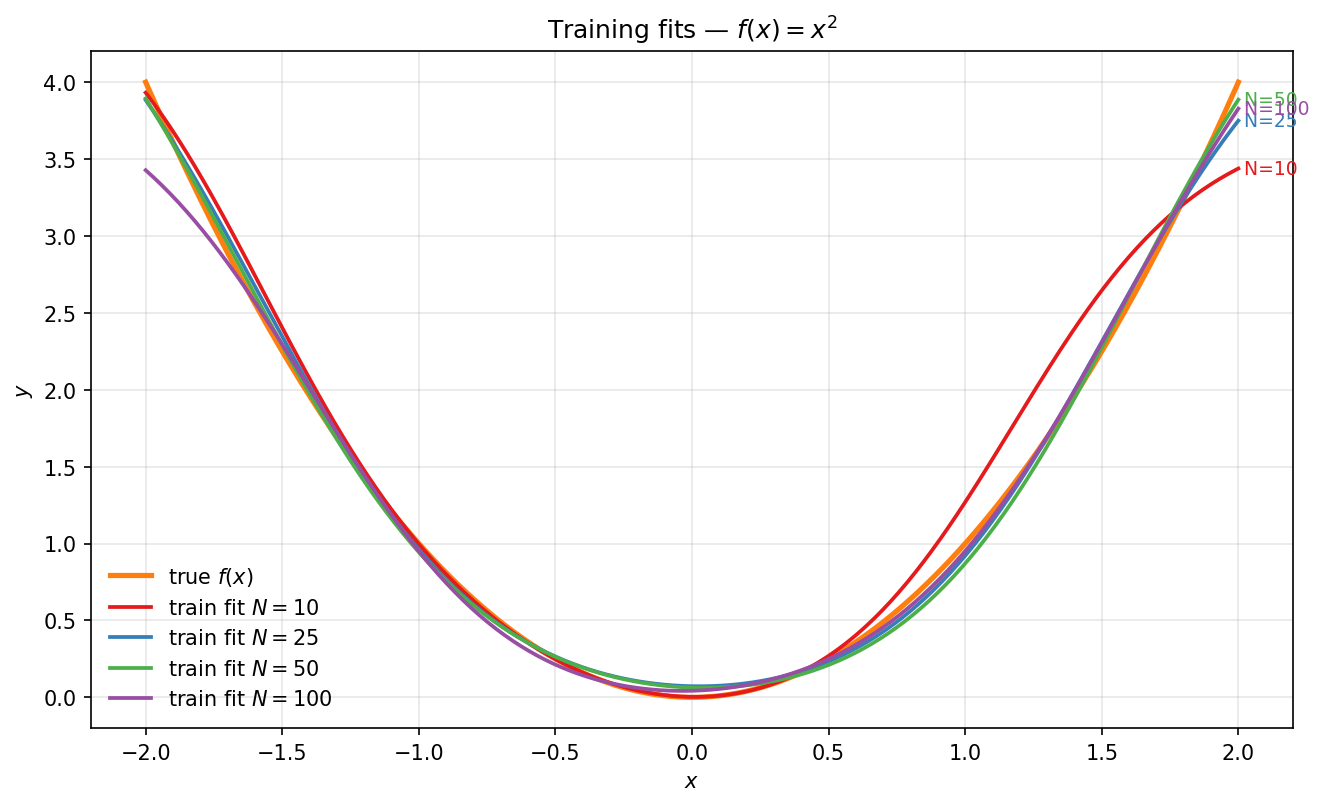
\includegraphics[width=0.92\textwidth]{figures/q1_train_square.png}
  \caption{Training view for $f(x)=x^{2}$: orange solid curve is the true
  $f(x)$; coloured curves are network fits for each training-set size $N$
  (same colour coding as the test plot).}
  \label{fig:q1train_sq}
\end{figure}

\begin{figure}[htbp]
  \centering
  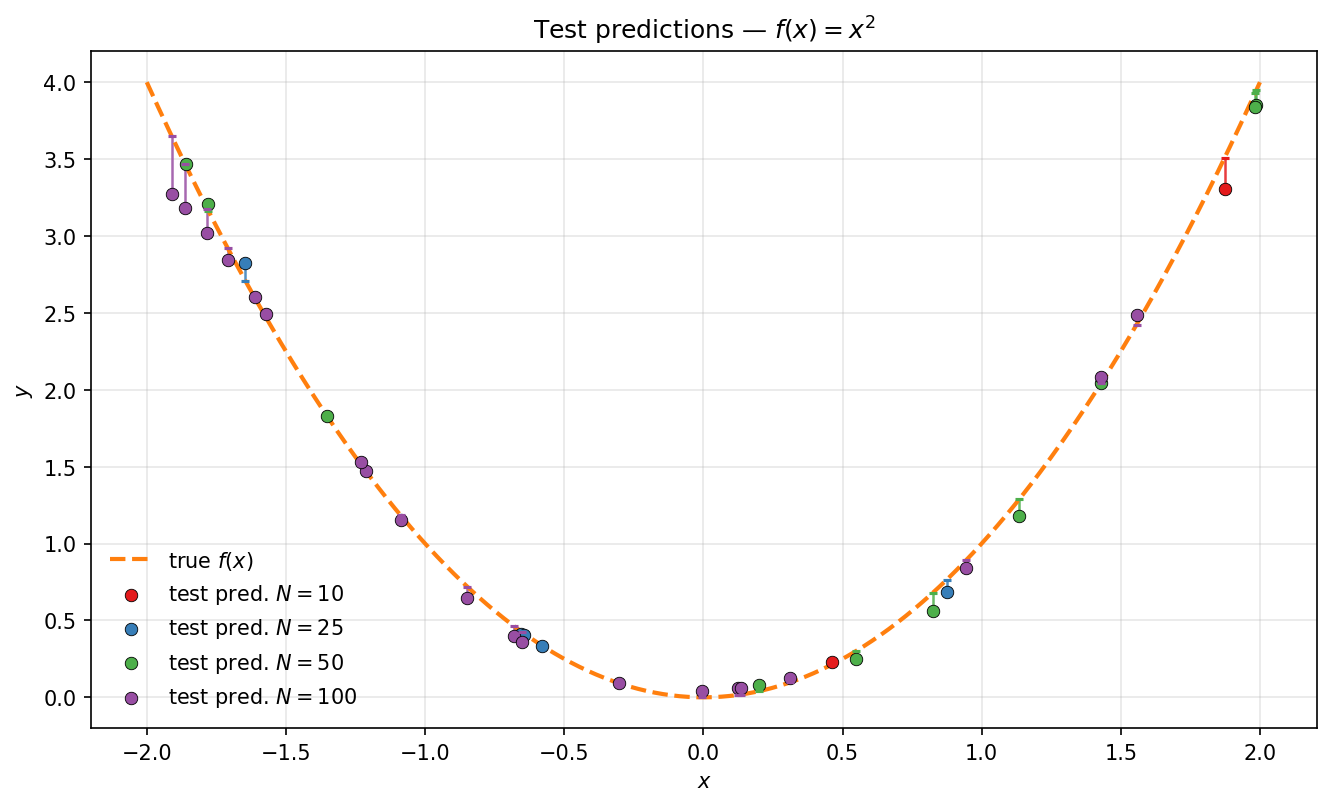
\includegraphics[width=0.92\textwidth]{figures/q1_test_square.png}
  \caption{Test view for $f(x)=x^{2}$: orange dotted curve is the true
  $f(x)$; coloured markers are network predictions on the held-out $20\%$
  test samples. Vertical bars (same colour per $N$) run from the true value
  to the prediction (residual / Excel-style error bars).}
  \label{fig:q1test_sq}
\end{figure}

\subsubsection*{Python implementation (modular core)}
\par\medskip
\noindent\begin{minipage}{\linewidth}
\begin{lstlisting}[caption={Forward pass, MSE, and training entry point}]
import numpy as np

def forward(x, w, b, W, b_out):
    h = np.tanh(x[:, None] * w[None, :] + b[None, :])
    return h @ W + b_out

def mse(y_hat, y_true):
    return float(np.mean((y_hat - y_true) ** 2))

# Fixed epochs (not until MSE = 0). 
\end{lstlisting}
\end{minipage}

\subsubsection*{Conclusion plots (MSE and time cost)}

\noindent\begin{minipage}{\linewidth}
\begin{center}
  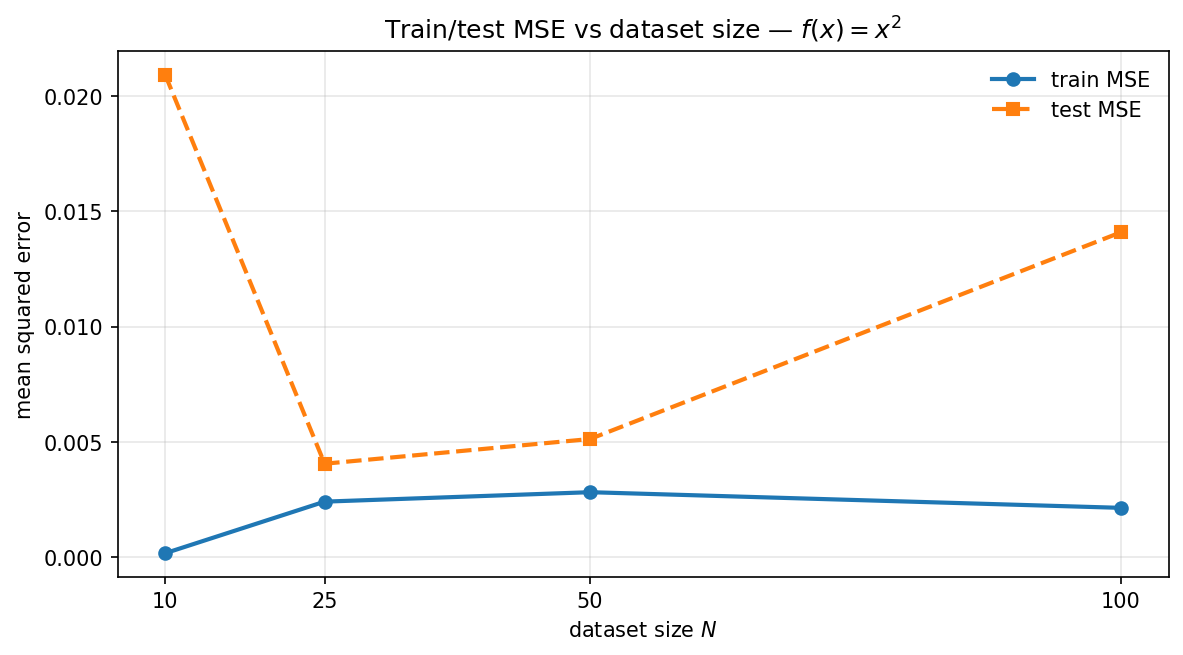
\includegraphics[width=0.92\textwidth]{figures/fit_square_errors.png}\\[0.8em]
  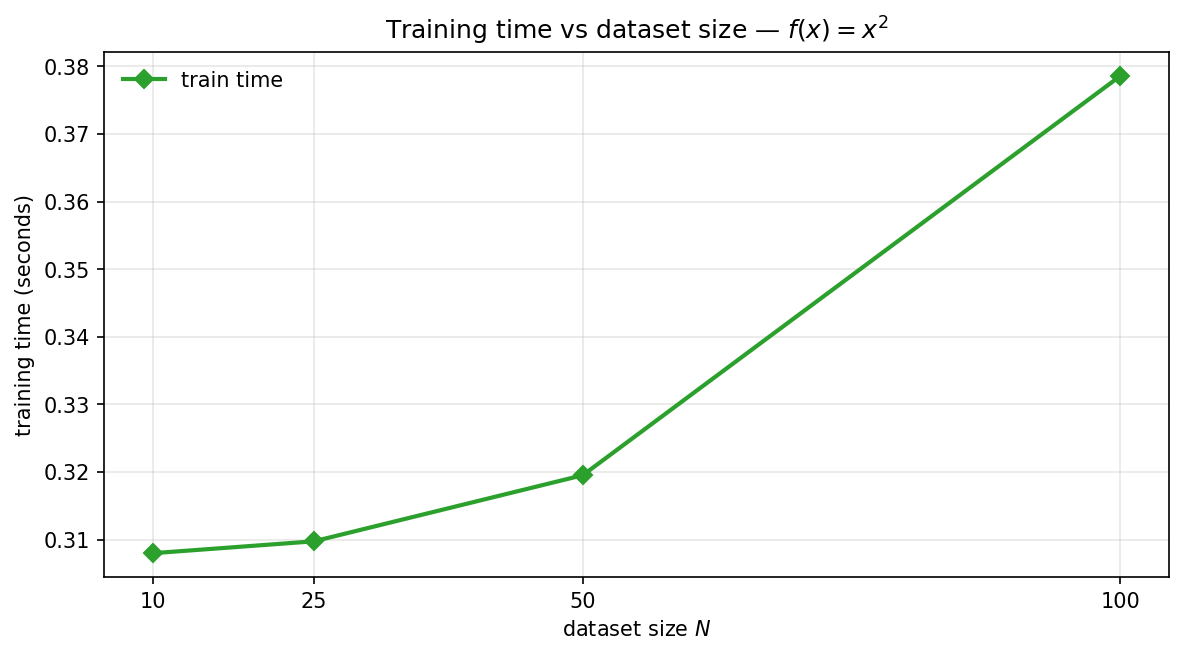
\includegraphics[width=0.92\textwidth]{figures/fit_square_time.png}
\end{center}
\captionof{figure}{Train/test MSE (top) and training wall-clock time (bottom)
versus dataset size for $f(x)=x^{2}$ under a fixed epoch budget.}
\label{fig:q1mse_time_sq}
\end{minipage}

\subsubsection*{Final learned weights}
\noindent\begin{minipage}{\linewidth}
\centering
\small
\begin{tabular}{lcccc}
\hline
Parameter & $N=10$ & $N=25$ & $N=50$ & $N=100$ \\
\hline
$w1$ & 1.4307 & -0.0079 & 0.0064 & 1.1487 \\
$b1$ & -1.6728 & 1.0832 & -1.4814 & -1.8338 \\
$w2$ & 1.3465 & 1.2673 & 1.1195 & 0.0442 \\
$b2$ & 0.9632 & -1.9263 & 1.8504 & 1.5016 \\
$w3$ & -1.5196 & -1.1888 & -1.2290 & -1.3283 \\
$b3$ & -2.4299 & -1.8812 & 1.9644 & -1.8412 \\
$W1$ & 2.0422 & 1.3332 & -2.2249 & 2.7916 \\
$W2$ & -0.5152 & 2.5378 & -2.9753 & 2.1109 \\
$W3$ & 2.0939 & 2.7647 & -2.7992 & 2.1923 \\
$b_out$ & 4.3518 & 4.0848 & 3.5800 & 2.8687 \\
\hline
\end{tabular}

\captionof{table}{Final trained parameters for $f(x)=x^{2}$ at each dataset size $N$.}
\label{tab:q1w_sq}
\end{minipage}

\subsubsection*{Analysis}
The training plot shows that using a larger dataset generally improves how
closely the network follows the true $f(x)=x^{2}$ curve. However, when the
dataset size is increased to $N=100$, the fitted curves start to deviate and
show overfitting behaviour. The MSE plot shows that, overall, the error trend
improves as more training data are used, while the test view indicates that
the $N=25$ set performed best for this target; further increasing the dataset
size raised the observed test error rate for this run.

\clearpage
\subsubsection*{Target $f(x)=\sin(x)$}

The same network and fixed-epoch MSE training are used, but the input domain
for this target is sampled in \textbf{degrees} on $x\in[-180^{\circ},180^{\circ}]$
and converted to radians before evaluating the sine and before feeding the
network
($x_{\mathrm{rad}}=\pi x_{\mathrm{deg}}/180$), so plots show a clear
period while $\tanh$ units are not saturated by degree-scale inputs.
Source:~\cite{CourseRepo}.

\begin{figure}[htbp]
  \centering
  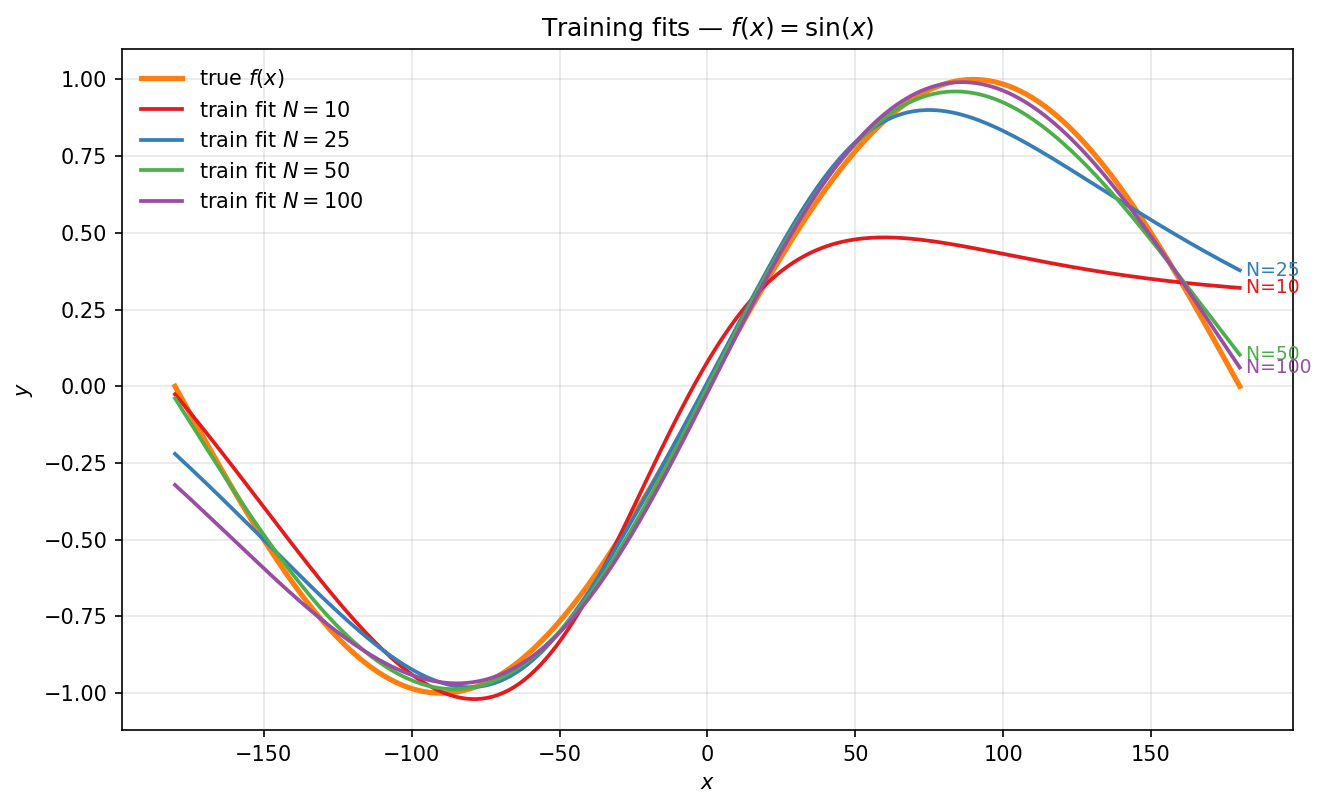
\includegraphics[width=0.92\textwidth]{figures/q1_train_sin.png}
  \caption{Training fits for $f(x)=\sin(x)$ with $x$ in degrees
  (converted to radians for the target).}
  \label{fig:q1train_sin}
\end{figure}

\begin{figure}[htbp]
  \centering
  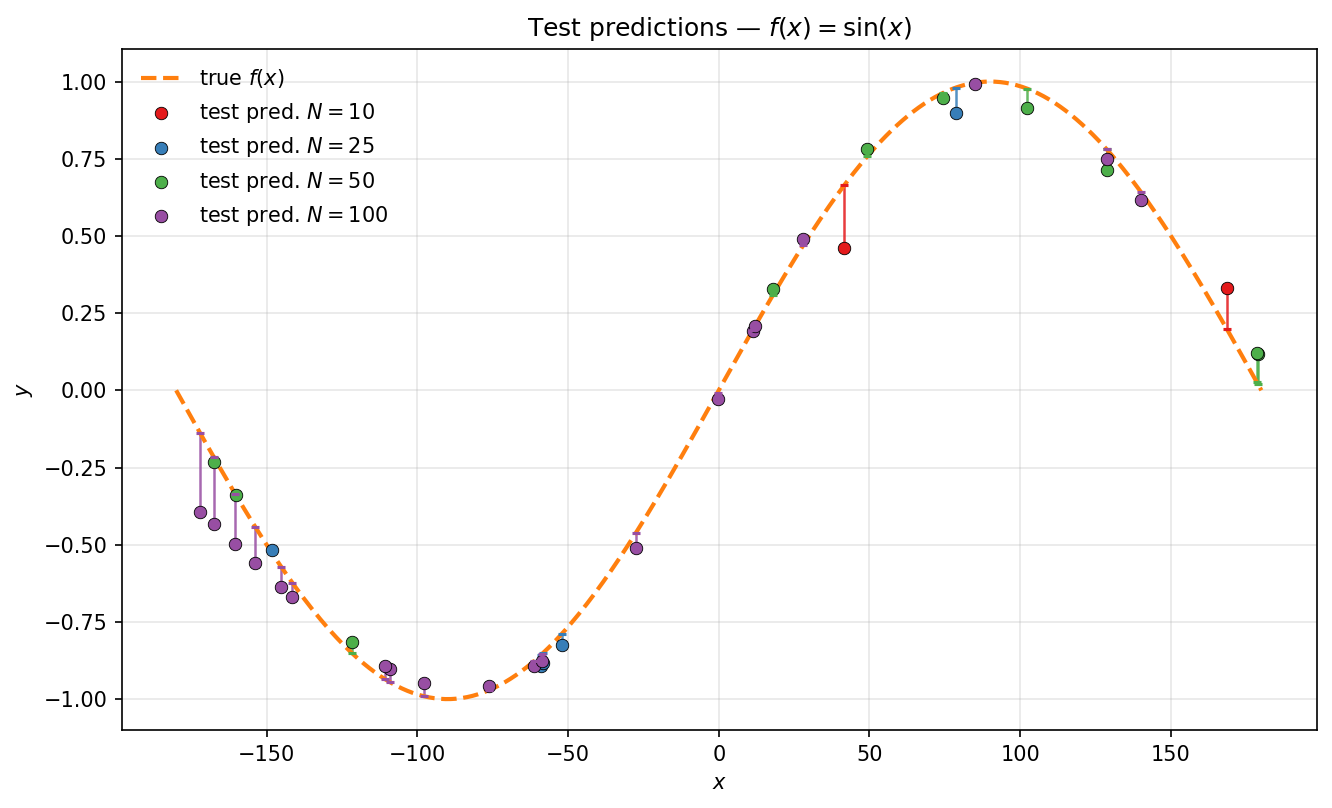
\includegraphics[width=0.92\textwidth]{figures/q1_test_sin.png}
  \caption{Test predictions with residual bars for $f(x)=\sin(x)$.}
  \label{fig:q1test_sin}
\end{figure}

\subsubsection*{Conclusion plots (MSE and time cost)}

\noindent\begin{minipage}{\linewidth}
\begin{center}
  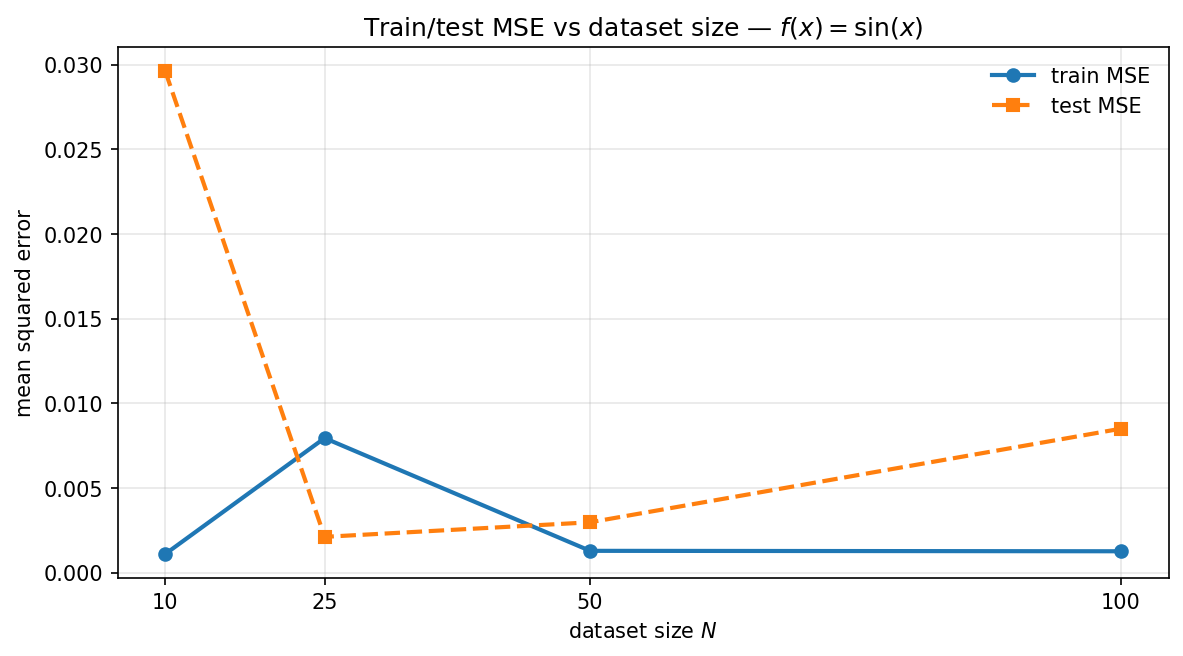
\includegraphics[width=0.92\textwidth]{figures/fit_sin_errors.png}\\[0.8em]
  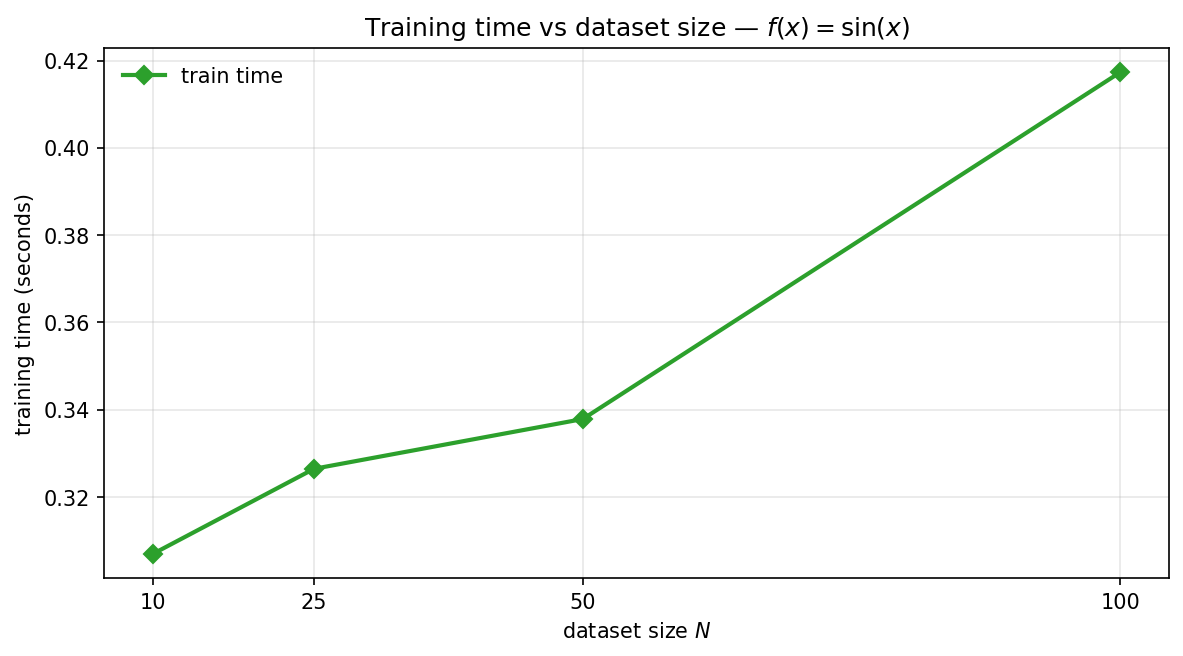
\includegraphics[width=0.92\textwidth]{figures/fit_sin_time.png}
\end{center}
\captionof{figure}{Train/test MSE (top) and training wall-clock time (bottom)
versus dataset size for $f(x)=\sin(x)$ under a fixed epoch budget.}
\label{fig:q1mse_time_sin}
\end{minipage}

\subsubsection*{Final learned weights}
\noindent\begin{minipage}{\linewidth}
\centering
\small
\begin{tabular}{lcccc}
\hline
Parameter & $N=10$ & $N=25$ & $N=50$ & $N=100$ \\
\hline
$w1$ & -0.6496 & 0.2715 & 0.5086 & 0.6894 \\
$b1$ & 0.6378 & 0.2113 & -1.3173 & 0.0033 \\
$w2$ & 1.0591 & 1.1875 & 0.5399 & -0.6209 \\
$b2$ & 0.4671 & -0.5209 & 1.5921 & 1.7443 \\
$w3$ & -0.4820 & -1.1292 & -0.6585 & -0.4918 \\
$b3$ & -1.1013 & -0.7453 & 0.0216 & -1.1461 \\
$W1$ & 0.2095 & -2.8783 & -1.6950 & 2.0665 \\
$W2$ & 1.5244 & 1.0871 & -1.7889 & 1.4735 \\
$W3$ & 1.6642 & -1.1662 & -2.1990 & 1.3662 \\
$b_out$ & 0.6301 & 0.3950 & 0.2234 & -0.2986 \\
\hline
\end{tabular}

\captionof{table}{Final trained parameters for $f(x)=\sin(x)$ at each dataset size $N$.}
\label{tab:q1w_sin}
\end{minipage}

\subsubsection*{Analysis}
Over this interval the training plot shows that for smaller datasets the
fitted curves do not match the true sinusoid well. Increasing the dataset
size finds better weights, so the learned behaviour becomes finer and closer
to the true curve. In particular, $N=50$ is a good approximation for this
target: increasing the data further mainly raises computational and timing
cost under our fixed-epoch schedule. The test results also show that for
$N=100$ the error increases and finding the weights takes longer than for
$N=50$, even though a longer budget might eventually do better---so the
computation cost must be understood as well. The train-time plot generally
rises with $N$, with some variability at $N=100$, where accuracy was still
worse: with the epoch budget exhausted the optimiser did not fully converge
and the large-data run appears to oscillate more. The MSE plot confirms this
analysis.

\clearpage
\subsubsection*{Target $f(x)=|x|^{2}$}

For real $x$, $|x|^{2}=x^{2}$, so this target produces the same parabola as
part~(a). The experiment is therefore not repeated.

\clearpage
% ---------------------------------------------------------------------------
% Question 2
% ---------------------------------------------------------------------------
\section*{Q2.\ Properties of the logistic sigmoid}

Show that the logistic sigmoid function satisfies
\(\sigma(-a)=1-\sigma(a)\) and that its inverse is given by
\(\sigma^{-1}(y)=\log\{y/(1-y)\}\).

The logistic sigmoid is defined by
\begin{equation}
  \sigma(a)=\frac{1}{1+e^{-a}}.
  \label{eq:sigmoiddef}
\end{equation}

\subsection*{(i)\ \(\sigma(-a)=1-\sigma(a)\)}

Substitute \(-a\) into~\eqref{eq:sigmoiddef}:
\begin{equation}
  \sigma(-a)=\frac{1}{1+e^{-(-a)}}=\frac{1}{1+e^{a}}.
\end{equation}
Next,
\begin{equation}
  1-\sigma(a)
    =1-\frac{1}{1+e^{-a}}
    =\frac{(1+e^{-a})-1}{1+e^{-a}}
    =\frac{e^{-a}}{1+e^{-a}}.
\end{equation}
Multiply the numerator and denominator of \(\sigma(-a)\) by \(e^{-a}\):
\begin{equation}
  \sigma(-a)
    =\frac{1}{1+e^{a}}\cdot\frac{e^{-a}}{e^{-a}}
    =\frac{e^{-a}}{e^{-a}+1}
    =\frac{e^{-a}}{1+e^{-a}}.
\end{equation}
Therefore
\begin{equation}
  \sigma(-a)=1-\sigma(a).
\end{equation}

\subsection*{(ii)\ Inverse \(\sigma^{-1}(y)=\log\{y/(1-y)\}\)}

Set \(y=\sigma(a)\) and solve for \(a\):
\begin{equation}
  y=\frac{1}{1+e^{-a}}.
\end{equation}
Multiply both sides by \(1+e^{-a}\):
\begin{equation}
  y\,(1+e^{-a})=1.
\end{equation}
Expand:
\begin{equation}
  y+y\,e^{-a}=1.
\end{equation}
Isolate the exponential:
\begin{align}
  y\,e^{-a}&=1-y,\\
  e^{-a}&=\frac{1-y}{y}.
\end{align}
Take the natural logarithm of both sides:
\begin{equation}
  -a=\log\!\left(\frac{1-y}{y}\right).
\end{equation}
Using \(-\log x=\log(1/x)\),
\begin{equation}
  a=\log\!\left(\frac{y}{1-y}\right).
\end{equation}
Hence
\begin{equation}
  \sigma^{-1}(y)=\log\!\left\{\frac{y}{1-y}\right\}.
\end{equation}

\clearpage
% ---------------------------------------------------------------------------
% Question 3
% ---------------------------------------------------------------------------
\section*{Q3.\ Consider two sets of outputs}

\begin{enumerate}
  \item[\textbf{Set~A:}] outcomes with \emph{minimum to low} entropy
  \item[\textbf{Set~B:}] outcomes with \emph{medium to high} entropy
\end{enumerate}

\subsection*{(a) Which set is more meaningful for decreasing unpredictable behaviour?}

\subsubsection*{Shannon entropy (analytical)}

Shannon's information theory defines the unpredictability of a discrete
random variable~\cite{He2018}. The Shannon measure of unpredictability is the
\textbf{Shannon entropy}. For a single outcome \(i\) with probability \(p_i\),
Shannon defined the \emph{surprise} (self-information) as
\begin{equation}
  \mathrm{information}(i)
    = \log_b\!\left(\frac{1}{p_i}\right)
    = -\log_b(p_i).
  \label{eq:selfinfo}
\end{equation}
Interpretation of~\eqref{eq:selfinfo}:
\begin{itemize}
  \item If \(p_i\) is close to \(1\) (a near-certain event), then
        \(\log(1/p_i)\) is close to \(0\) --- almost no information/surprise.
  \item If \(p_i\) is close to \(0\) (a rare event), then
        \(\log(1/p_i)\) is large --- a large amount of information/surprise.
\end{itemize}

For \emph{many} outcomes, the entropy of the full distribution is the
\textbf{probability-weighted sum} of these surprises:
\begin{equation}
  H(X)
    = \sum_{i} p_i \,\mathrm{information}(i)
    = \sum_{i} p_i \bigl(-\log_b p_i\bigr)
    = -\sum_{i} p_i \log_b p_i,
  \label{eq:shannon}
\end{equation}
where \(p_i\) is the probability of outcome \(i\) and the base \(b\) chooses
the unit (bits when \(b=2\)). Equation~\eqref{eq:shannon} is the general
multi-outcome formula used for Set~A and Set~B below.

\paragraph{Special case (two outcomes).}
For a Bernoulli system with probabilities \(p\) and \(1-p\),~\eqref{eq:shannon}
reduces to the \textbf{binary entropy}
\begin{equation}
  H(p) = -p\log_2 p - (1-p)\log_2(1-p).
\end{equation}
\(H(p)\) is \emph{low} when \(p\) is near \(0\) or near \(1\) (highly
predictable outcomes) and reaches its \emph{maximum} at \(p=0.5\) (maximum
randomness). Thus ``minimum to low entropy'' corresponds to probability mass
concentrated on nearly certain outcomes, while ``medium to high entropy''
corresponds to more uniformly uncertain outcomes.

\subsubsection*{Figures}

Figure~\ref{fig:binary} shows the binary-entropy special case \(H(p)\).
Entropy is smallest near the extremes of \(p\).

\begin{figure}[htbp]
  \centering
  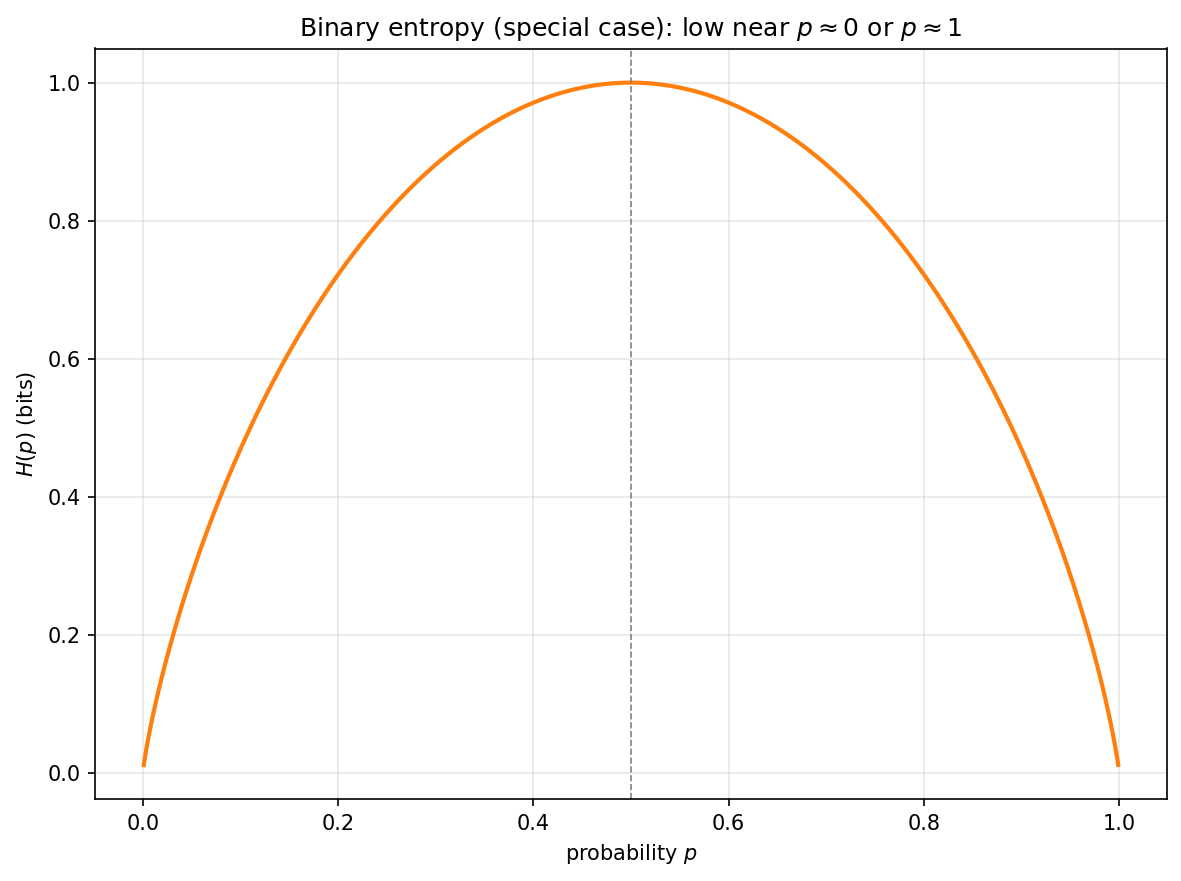
\includegraphics[width=0.85\textwidth]{figures/binary_entropy.png}
  \caption{Binary Shannon entropy \(H(p)\) versus probability \(p\)
  (special case of two outcomes). Low entropy occurs for very small or
  very large \(p\).}
  \label{fig:binary}
\end{figure}

To connect~\eqref{eq:shannon} to Set~A and Set~B, we form two sample sets
whose outcomes are integers from \(1\) to \(10\) (size \(N=100\)):
\begin{itemize}
  \item \textbf{Set~A:} draws are random, but a few numbers appear much more
        often (peaked frequencies \(\Rightarrow\) low entropy).
  \item \textbf{Set~B:} draws are nearly uniform, so the same number rarely
        dominates (spread frequencies \(\Rightarrow\) high entropy).
\end{itemize}
Empirical probabilities are \(p_i = n_i/N\). Importantly:
\begin{itemize}
  \item The \textbf{top histograms} show only \emph{counts} (how often each
        outcome appears). They are \emph{not} an entropy curve.
  \item \textbf{Entropy} is a \emph{single number} for each whole set,
        \(H=-\sum_i p_i\log_2 p_i\), shown in the \textbf{bottom panel} of
        Figure~\ref{fig:sets}.
\end{itemize}

\begin{figure}[htbp]
  \centering
  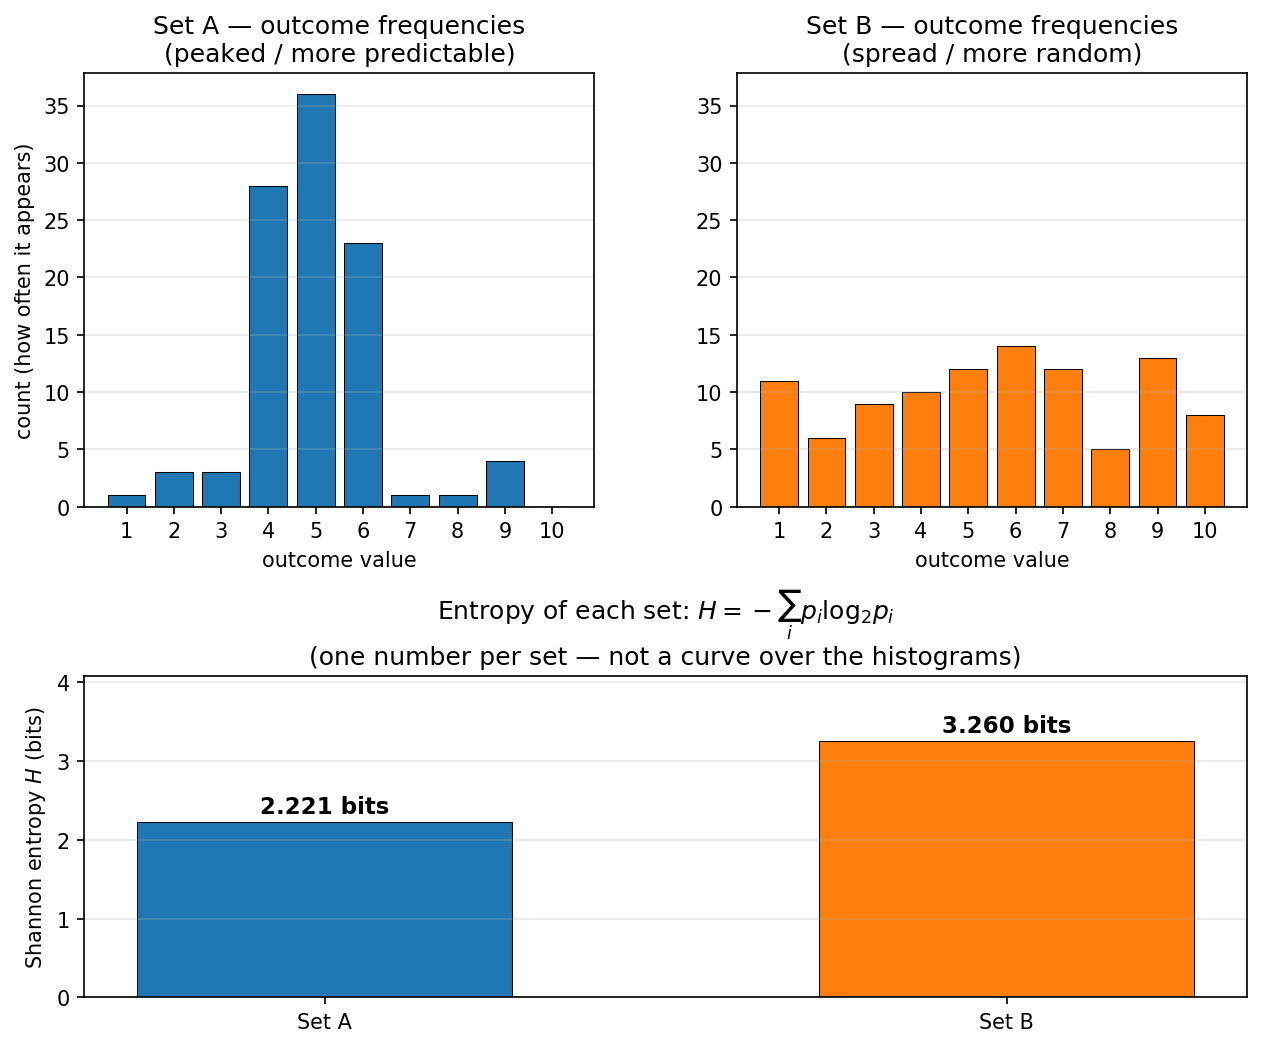
\includegraphics[width=0.95\textwidth]{figures/set_ab_entropy.png}
  \caption{Top: outcome frequencies for Set~A and Set~B (values 1--10).
  Bottom: Shannon entropy of each set (one bar per set). The histograms
  describe the data; the bottom panel is where entropy is compared.}
  \label{fig:sets}
\end{figure}

\subsubsection*{Conclusion}

Entropy is a direct measure of randomness / unpredictability. To
\emph{reduce} unpredictable behaviour we need outcomes that are as
predictable as possible --- concentrated probability mass and
\textbf{low Shannon entropy}. From~\eqref{eq:selfinfo},~\eqref{eq:shannon},
and Figures~\ref{fig:binary}--\ref{fig:sets}, that regime is exactly
\textbf{Set~A}. Set~B corresponds to greater uncertainty and is less
suitable if the design goal is to reduce randomness.

\noindent\textit{Note.} Full plotting scripts and libraries are in the course
repository~\cite{CourseRepo}.


\subsubsection*{Python Implementation}
\par\medskip
\noindent\begin{minipage}{\linewidth}
\begin{lstlisting}[caption={Shannon entropy and binary entropy}]
import numpy as np

def shannon_entropy(probs, base=2.0):
    """H = -sum p_i log_b(p_i)  (weighted sum over many outcomes)."""
    p = np.asarray(probs, dtype=float)
    p = p / p.sum()
    nz = p > 0
    return float(-(p[nz] * (np.log(p[nz]) / np.log(base))).sum())

def binary_entropy(p, base=2.0):
    """Special case: H(p) for Bernoulli(p); low near p=0 or p=1."""
    p = np.clip(np.asarray(p, dtype=float), 0.0, 1.0)
    h = np.zeros_like(p, dtype=float)
    mid = (p > 0) & (p < 1)
    pm = p[mid]
    h[mid] = -(pm * np.log(pm) + (1 - pm) * np.log(1 - pm)) / np.log(base)
    return h
\end{lstlisting}
\end{minipage}

\clearpage
% ---------------------------------------------------------------------------
% Question 4
% --------------------------------------------------------------------------
\section*{Q4.\ Normal distribution and maximum entropy}

If we know the mean \(\mu\) and standard deviation \(\sigma\), is it true that
the Normal (Gaussian) distribution has the maximum entropy?

\subsubsection*{Differential entropy}

For a continuous random variable with density \(p(x)\), Shannon's discrete
sum becomes an integral the \textbf{differential entropy}
\begin{equation}
  H(X) = -\int_{-\infty}^{\infty} p(x)\,\log p(x)\,dx
  \label{eq:diffent}
\end{equation}
This is the continuous
analogue of~\eqref{eq:shannon}. Standard results in information theory show
that, among all continuous densities that share a fixed mean \(\mu\) and
fixed variance \(\sigma^2\), the Gaussian density uniquely maximises
\(H(X)\)~\cite{Blahut2002}.

\subsubsection*{Entropy of a Gaussian}

For \(X\sim\mathcal{N}(\mu,\sigma^2)\) the integral~\eqref{eq:diffent}
evaluates in closed form to
\begin{equation}
  H(X) = \tfrac{1}{2}\log_2\!\bigl(2\pi e\,\sigma^2\bigr)
  \quad\text{(bits)}.
  \label{eq:gaussH}
\end{equation}
Two observations follow immediately from~\eqref{eq:gaussH}:
\begin{itemize}
  \item \(H(X)\) depends only on the variance \(\sigma^2\), \emph{not} on the
        mean \(\mu\). Entropy measures unpredictability (spread), not where
        the bell curve is centred. Shifting the curve left or right does not
        change how uncertain the outcome is.
  \item As \(\sigma\to 0\) (a very narrow spike) the entropy becomes very
        small: you are almost certain of the value. As \(\sigma\) grows
        (a very wide curve) the entropy grows: values can land almost
        anywhere, so uncertainty is high.
\end{itemize}

\subsubsection*{Maximum-entropy principle}

The entropy under given constraints is maximized by the Normal distribution.
\begin{enumerate}
  \item \(\displaystyle\int p(x)\,dx = 1\) (a valid density),
  \item \(\displaystyle\mathbb{E}[X]=\mu\) and
        \(\displaystyle\mathrm{Var}(X)=\sigma^2\) (known mean and spread),
\end{enumerate}
Equivalently: among all continuous
distributions that share the same \(\mu\) and \(\sigma^2\), the Gaussian
is the one with the \textbf{highest} differential entropy. Any other shape
with the same mean and variance (skewed, multimodal, truncated, \ldots)
secretly encodes \emph{extra} structure beyond what \(\mu\) and \(\sigma^2\)
alone justify, and that extra structure \emph{reduces} entropy. 
Gaussian is therefore the ``least additional-assumption'' choice consistent
with those two facts the \textbf{maximum entropy principle}~\cite{Blahut2002}.

\subsubsection*{Illustration (same \(\mu,\sigma^2\), different shapes)}

Figure~\ref{fig:maxent} fixes \(\mu=0\) and \(\sigma=1\) and plots three
densities that all have this mean and variance: Gaussian, Laplace, and
Uniform. The left panel shows the shapes; the right panel shows their
differential entropies. 

\begin{figure}[htbp]
  \centering
  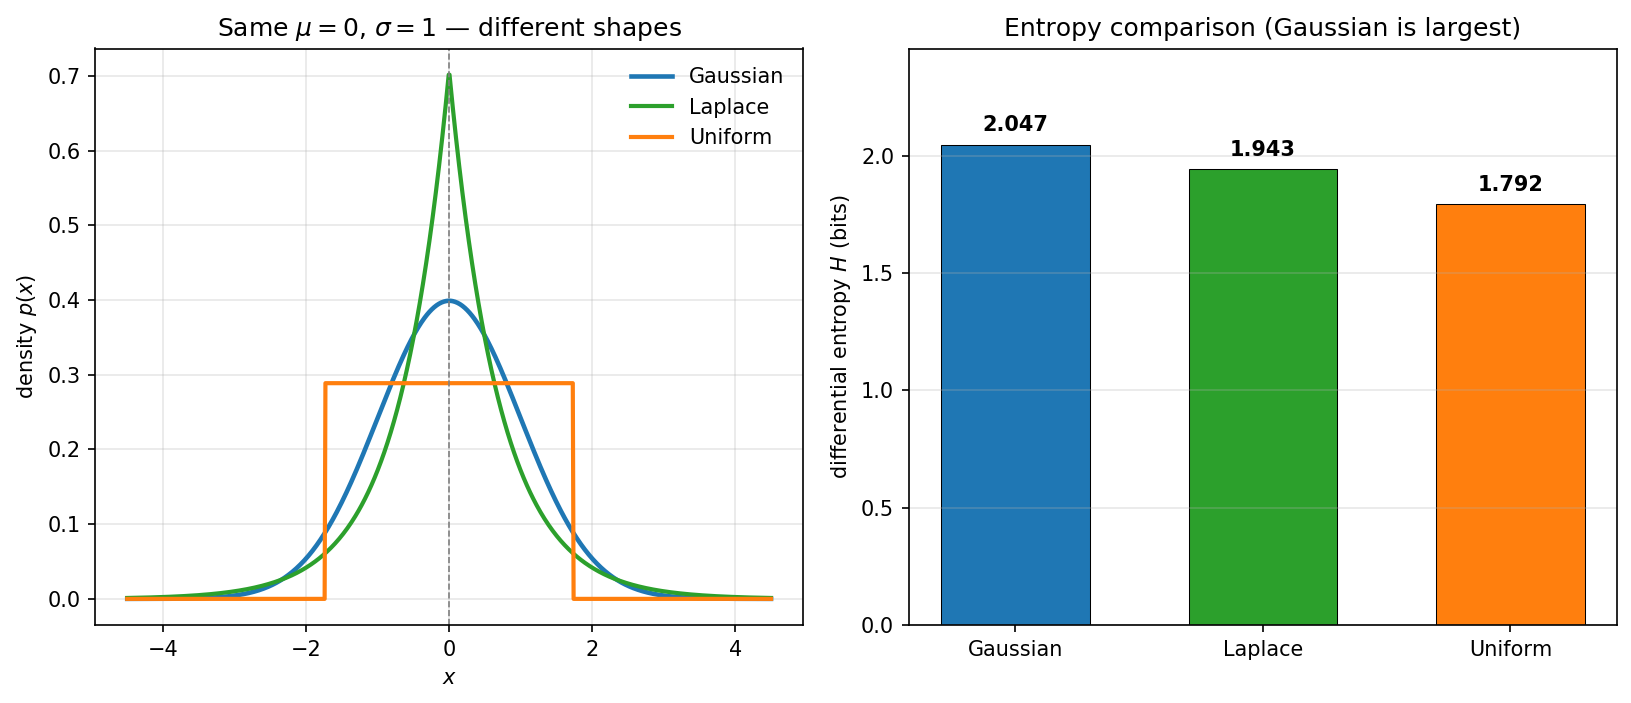
\includegraphics[width=0.98\textwidth]{figures/maxent_gaussian.png}
  \caption{Left: three PDFs with identical \(\mu\) and \(\sigma^2\).
  Right: differential entropy of each. The Gaussian has the largest \(H\);
  the other shapes add extra structure (sharper peak or hard cut-offs) and
  therefore lower entropy.}
  \label{fig:maxent}
\end{figure}


\clearpage
% ---------------------------------------------------------------------------
% Question 5
% ---------------------------------------------------------------------------
\section*{Q5.\ Find and plot the derivatives of (a)~ReLU, (b)~Sigmoid, and
(c)~Hyperbolic Tangent functions.}

% ===========================================================================
\subsection*{ (a) ReLU }
% ===========================================================================

\subsubsection*{Analytical Form}

The Rectified Linear Unit (ReLU) is defined as
\begin{equation}
  \mathrm{ReLU}(x) = \max(0, x) =
  \begin{cases}
    0, & x < 0, \\
    x, & x \geq 0.
  \end{cases}
\end{equation}
Differentiating piecewise (taking the subgradient at \(x = 0\) to be \(0\),
as is common in practice) yields
\begin{equation}
  \mathrm{ReLU}'(x) =
  \begin{cases}
    0, & x \leq 0, \\
    1, & x > 0.
  \end{cases}
\end{equation}

Figure 1 shows the ReLU activation function and its derivative.
\subsubsection*{Plot}
The derivative in python code is simple finite check in the limits given while for the derivative at Zero its taken as 0.
\begin{figure}[htbp]
  \centering
  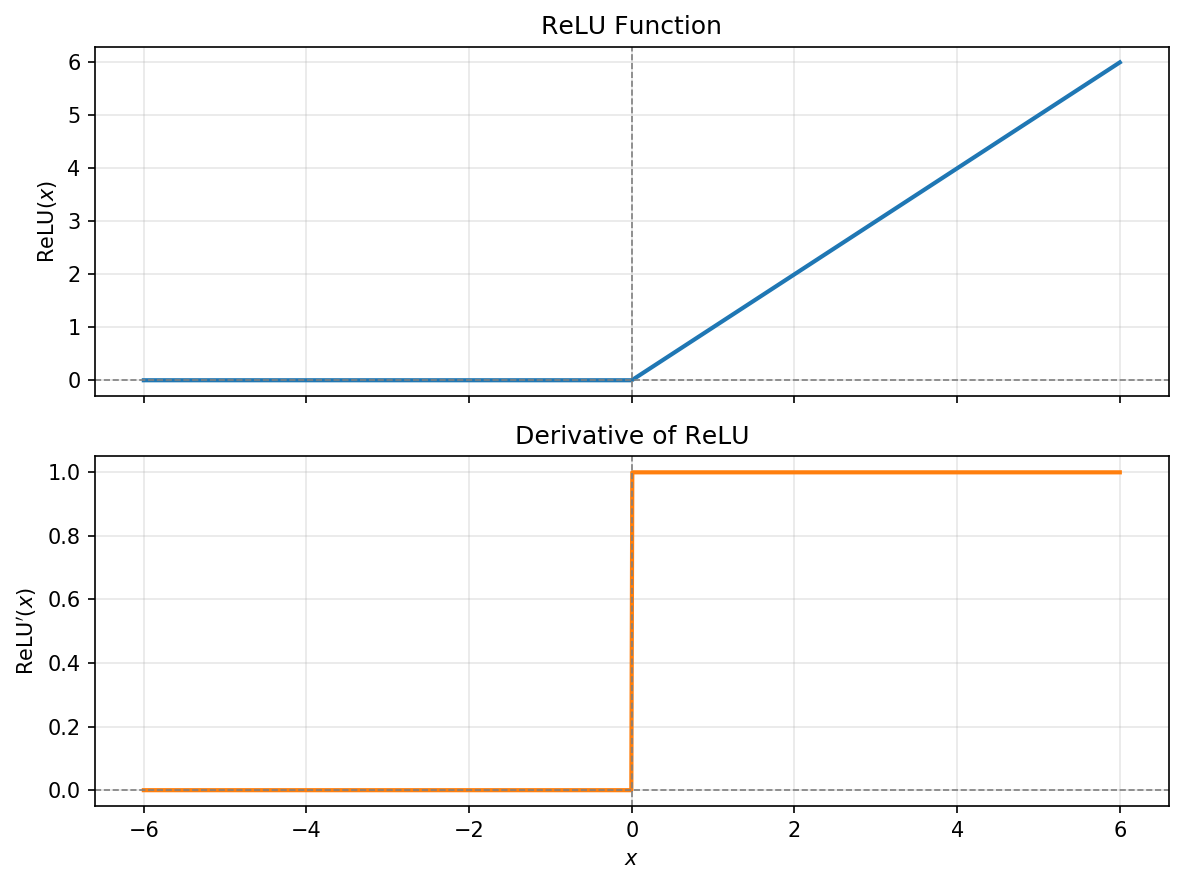
\includegraphics[width=0.85\textwidth]{figures/relu.png}
  \caption{ReLU activation (top) and its derivative (bottom).}
  \label{fig:relu}
\end{figure}

\subsubsection*{Python Implementation}
\noindent\begin{minipage}{\linewidth}
For the computation of derivatives we have used the NumPy library.

\vspace{0.6em}
\begin{lstlisting}[caption={ReLU and its derivative}]
import numpy as np
def relu(x):
    return np.maximum(0.0, x)

def relu_derivative(x):
    return (x > 0).astype(float)
\end{lstlisting}
\end{minipage}

\clearpage
% ===========================================================================
\subsection*{ (b) Sigmoid }
% ===========================================================================

\subsubsection*{Analytical Form}

The logistic sigmoid is
\begin{equation}
  \sigma(x) = \frac{1}{1 + e^{-x}}.
\end{equation}
Differentiating with respect to \(x\):
\begin{align}
  \sigma'(x)
    &= \frac{e^{-x}}{(1 + e^{-x})^2}
     = \frac{1}{1 + e^{-x}} \cdot \frac{e^{-x}}{1 + e^{-x}}
     = \sigma(x)\,(1 - \sigma(x)).
\end{align}
Thus
\begin{equation}
  \sigma'(x) = \sigma(x)\,(1 - \sigma(x)).
\end{equation}

\subsubsection*{Figure}
Figure 2 shows the Sigmoid activation function and its derivative. Chain rule has been used to find the derivative.
\begin{figure}[htbp]
  \centering
  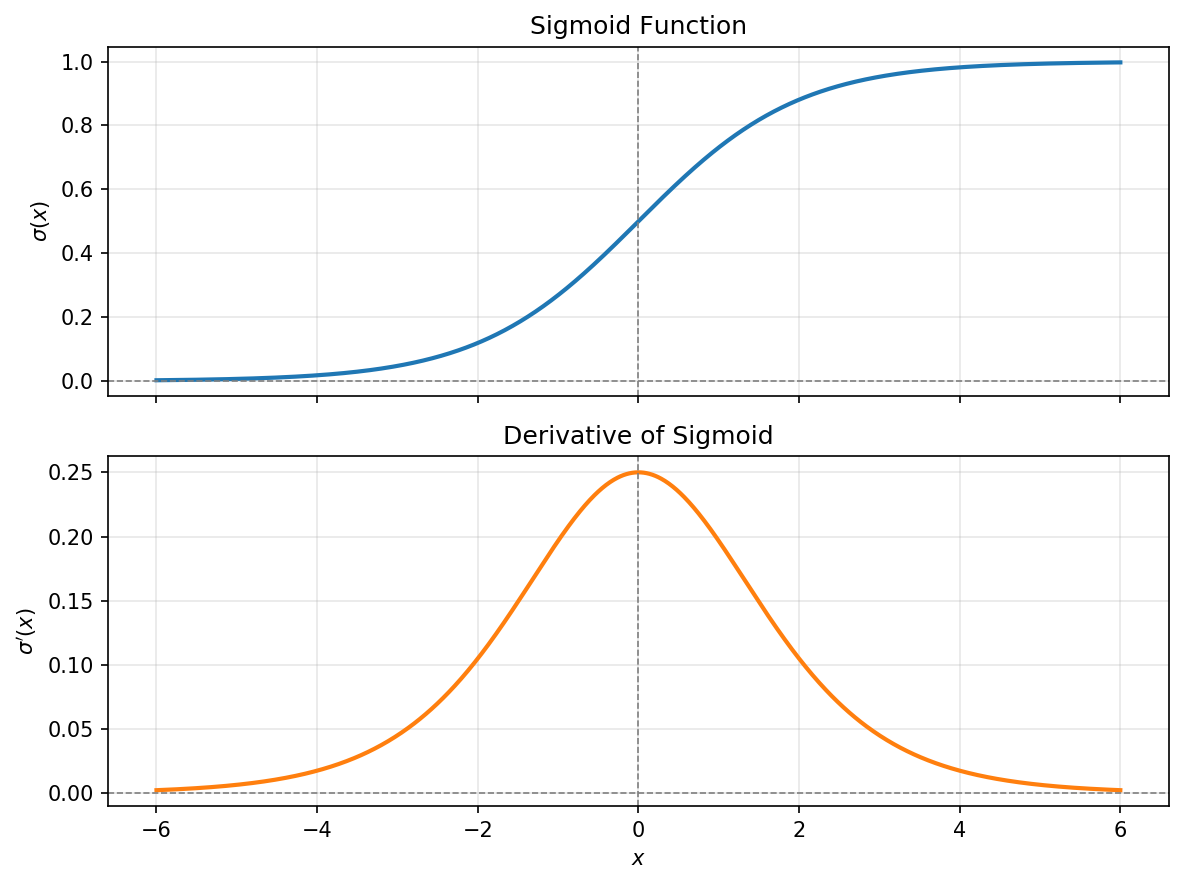
\includegraphics[width=0.85\textwidth]{figures/sigmoid.png}
  \caption{Sigmoid activation (top) and its derivative (bottom).}
  \label{fig:sigmoid}
\end{figure}

\subsubsection*{Python Implementation}
\par\medskip
\noindent\begin{minipage}{\linewidth}
\begin{lstlisting}[caption={Sigmoid and its derivative}]
import numpy as np

def sigmoid(x):
    return 1.0 / (1.0 + np.exp(-x))

def sigmoid_derivative(x):
    s = sigmoid(x)
    return s * (1.0 - s)
\end{lstlisting}
\end{minipage}

\clearpage
% ===========================================================================
\subsection*{ (c) Hyperbolic Tangent }
% ===========================================================================

\subsubsection*{Analytical Form}

The hyperbolic tangent is
\begin{equation}
  \tanh(x) = \frac{e^{x} - e^{-x}}{e^{x} + e^{-x}}
           = \frac{\sinh(x)}{\cosh(x)}.
\end{equation}
Its derivative follows from the quotient rule (or the identity
\(\frac{d}{dx}\tanh x = \mathrm{sech}^2 x\)):
\begin{equation}
  \tanh'(x) = 1 - \tanh^2(x) = \mathrm{sech}^2(x).
\end{equation}

\subsubsection*{Figure}
Figure 3 shows the Hyperbolic Tangent activation function and its derivative. Chain rule has been used to find the derivative.

\begin{figure}[htbp]
  \centering
  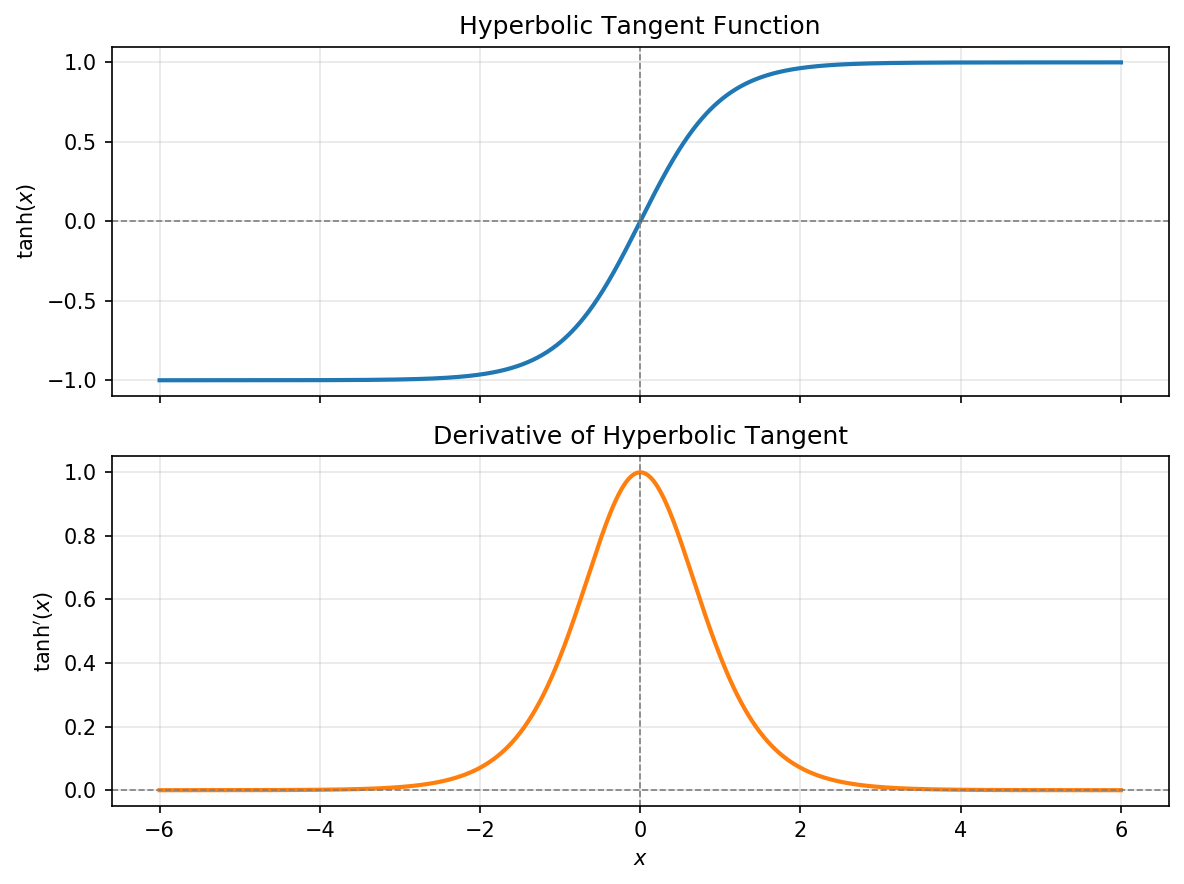
\includegraphics[width=0.85\textwidth]{figures/tanh.png}
  \caption{Hyperbolic tangent activation (top) and its derivative (bottom).}
  \label{fig:tanh}
\end{figure}

\subsubsection*{Python Implementation}
\par\medskip
\noindent\begin{minipage}{\linewidth}
\begin{lstlisting}[caption={Hyperbolic tangent and its derivative}]
import numpy as np

def tanh_fn(x):
    return np.tanh(x)

def tanh_derivative(x):
    t = np.tanh(x)
    return 1.0 - t**2
\end{lstlisting}
\end{minipage}

% ---------------------------------------------------------------------------
% References
% ---------------------------------------------------------------------------
\begin{thebibliography}{9}

\bibitem{He2018}
Q.~Peter He,
\textit{Information Entropy based Indices for Variable Selection Performance
Assessment},
in Mario~R.\ Eden, Marianthi~G.\ Ierapetritou, Gavin~P.\ Towler (Eds.),
\textit{Computer Aided Chemical Engineering}, Elsevier, Volume~44, 2018,
pp.~2281--2286,
ISSN~1570-7946, ISBN~9780444642417,
\url{https://doi.org/10.1016/B978-0-444-64241-7.50375-X}.

\bibitem{CourseRepo}
Z.~Khan,
\textit{Deep Learning Course} (source code and scripts),
GitHub repository,
\url{https://github.com/ZawarKhan97/Deep_Learning_Course}.

\bibitem{Blahut2002}
R.~E.\ Blahut,
\textit{Information Theory and Coding},
in Wendy~M.\ Middleton, Mac~E.\ Van Valkenburg (Eds.),
\textit{Reference Data for Engineers} (Ninth Edition), Newnes, 2002,
pp.~25-1--25-31, ISBN~9780750672917,
\url{https://doi.org/10.1016/B978-075067291-7/50027-3}.

\end{thebibliography}

\end{document}
